\documentclass[a4paper,11pt]{article}
%\documentclass[a4paper,9pt,landscape]{article}
\usepackage[english]{babel}
%\usepackage[utf8]{inputenc}
\usepackage{graphicx}
\usepackage{fullpage}
\usepackage{amsmath}
\usepackage{pdfpages}
\usepackage{listings}
\usepackage{color}
\usepackage{multicol}
\usepackage{fancyhdr}
\usepackage[top=1.5cm, bottom=4cm, left=2.5cm, right=2.5cm]{geometry}
\usepackage{hyperref}
\usepackage{verbatim}
\setlength{\voffset}{-9pt}
%\setlength{\hoffset}{-1in}
%\setlength{\marginparsep}{0.5cm}


\setlength{\parindent}{1cm}
%\setlength{\parskip}{-0.1cm}
%\setlength{\columnseprule}{0.4pt}
\setlength{\footskip}{0.5cm}
\setlength{\headheight}{15pt}
\setlength{\headsep}{2cm}

\fancypagestyle{tcr}{%
  \fancyhf{} %clear all headers and footers fields
  \fancyhead[R]{\thepage}
  \fancyhead[L]{\textbf{Lab No 1 TDDC78}}
  \renewcommand{\headrulewidth}{0.4pt}
}

\definecolor{dkgreen}{rgb}{0,0.6,0}
\definecolor{gray}{rgb}{0.5,0.5,0.5}
\definecolor{mauve}{rgb}{0.58,0,0.82}
\lstset{
  title=\lstname,
  frame=t,
  %aboveskip=-0.5cm, 
  %belowskip=0pt,
  basicstyle=\footnotesize\ttfamily,
  keywordstyle=\color{blue},          % keyword style
  commentstyle=\color{dkgreen},       % comment style
  stringstyle=\color{mauve},         % string literal style
  showstringspaces=false,         % underline spaces within strings
  tabsize=2,
  language=C,
  title=\caption,
  %xleftmargin=-1cm
}


\begin{document}
%% title stuff
\title{Lab No 3 TDDC78}
\author{Linus Mellberg (linme560) \and Oskar Aagaard (oskaa489)}
\date{\today}
\maketitle
\pagebreak
%\setcounter{page}{1}
%\begin{multicols}{2}
\thispagestyle{tcr}
\pagestyle{tcr}
%\tableofcontents

\section{Stationary Heat Conduction Using OpenMP}



The averaging filter works by convoluting the input image with a gaussian filter kernel.
This will do a weighted average on the pixel and the pixels surrounding it.
Since the gaussian kernel is symmetric the the calculation can be simplified, this makes the problem linear in the radius of the kernel.
\subsection{Description of the program}
The program uses the MPI framework for communication between the processes.
Parallelization is done by splitting the picture into equal regions along the y-axis.
Each process then apply the filter on the region that is given to it. 
Since the filter does averaging on the neighbouring pixels each process needs more data than the pixels which it filters.
This makes it neccesary to send more data to each process than the data that belongs to the region which it filters.

The process with rank 0 reads the image from disk.
When this is done it broadcast the dimension of the picture.
Every process then calculates how the picture is divided into regions and shared between the processes.
When this is done the rank 0 process send the data to the processes, each process gets all data needed to do its own filtering.
As soon as a process has recieved its data it will start applying the filter to it.
The rank 0 process also gets a region of the image and start processing as soon as possible.
When the processes are done with the filtering a \emph{MPI\_Gatherv} operation is performed to collect all the data at the rank 0 process.
This process then writes the filtered image to disk.

At first the nonblocking send was used to distribute data to the processes.
When the program was analyzed with traceanalyzer it was discovered that this is not a good thing to do.
The nonblocking send does not send the data immediately.
It seems that what is done is put the data into a buffer and send this when another MPI call is waiting to complete.
The result of this behavoiur is that the root process completes its own filtering before sending any data to the other processes.
This makes all the other processes idle while the root process filter the data given to it, this effectively doubles the execution time of the program.
When using the blocking send operation all data is sent before any filtering and the non-root processes are only idle when data is read and written to disk.

\subsection{Result and graphs}

\clearpage

\begin{comment}
%bulletlist
\paragraph\noindent\textbf{Overview of the linear program}
\begin{itemize}
\renewcommand{\labelitemi}{$\bullet$}
\item Load image from disk
\item Calculate average RGB sum
\item Calculate output image
\item Write image to disk
\end{itemize}

%picture import
\begin{figure}[!h]
  \caption{Run times related to number of cores for the different images.}
  \label{runtime_vs_cores}
  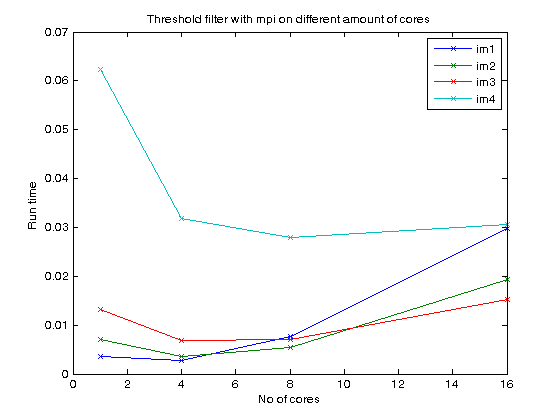
\includegraphics[scale=0.9]{../plots/runtimevscoresthres.png}
\end{figure}

%table
\begin{table}[h!]
  \caption{$MPixels/Second$ when running with different amount of threads and on different data.}
  \label{mpixelspersecond}
  \begin{tabular}[h]{|l|l|l|l|l|l|}
    \hline
                      & 1      & 2      & 4      & 8      & 16\\
    \hline
    im1.ppm           & 135.41 & 183.31 & 184.94 & 68.89  & 21.77\\ 
    im2.ppm           & 150.01 & 209.17 & 274.71 & 201.65 & 63.15\\ 
    im3.ppm           & 146.25 & 209.72 & 274.44 & 275.62 & 138.23\\ 
    im4.ppm           & 145.07 & 212.56 & 286.41 & 332.90 & 297.42\\
    \hline
  \end{tabular}
\end{table}

%citation from bibliography
\cite{fenwick}

%bibliography
\clearpage
\begin{thebibliography}{9}
  \bibitem{fenwick}
    Binary Indexed Trees,
    \emph{Algortihmist}.\\
    \url{http://community.topcoder.com/tc?module=Static\&d1=tutorials\&d2=binaryIndexedTrees}
  \bibitem{ppm}
    Mark Nelson,
    \emph{Arithmetic Coding + Statistical Modeling = Data Compression}, 1991.\\
    \url{http://marknelson.us/1991/02/01/arithmetic-coding-statistical-modeling-data-compression/}
  \bibitem{ppmc}
    PPM
    \url{http://www.cs.ucf.edu/courses/cap5015/ppm.pdf}

\end{thebibliography}a

%sourcecode listing
\lstinputlisting[caption=mpiblur.c]{../mpiblur.c}
\end{comment}

\clearpage
\section{Source code}
Files that are included but not listed here were downloaded from the course webpage and not modified.

\end{document}
